\documentclass[12pt]{article}
\usepackage{sbc-template}
\usepackage{enumerate}
\usepackage{hyperref} 
\usepackage{url} 
\usepackage{tikz}
\usepackage[utf8]{inputenc}
\usepackage[brazil]{babel}
\usepackage[T1]{fontenc}
\usepackage[scaled=0.85]{beramono}
\usepackage{csquotes}
\usepackage{listings}
\usepackage{color}
\usepackage{amsmath}
\usepackage{graphicx}
\renewcommand\lstlistingname{C\'odigo}
\setlength\parindent{20pt}

\usetikzlibrary{decorations.pathreplacing,calc}
\newcommand{\tikzmark}[1]{\tikz[overlay,remember picture] \node (#1) {};}

\newcommand\numberthis{\addtocounter{equation}{1}\tag{\theequation}}

\newcommand*{\AddNote}[4]{%
    \begin{tikzpicture}[overlay, remember picture]
        \draw [decoration={brace,amplitude=0.4em},decorate,black]
            ($(#3)!([yshift=1.5ex]#1)!($(#3)-(0,1)$)$) --  
            ($(#3)!(#2)!($(#3)-(0,1)$)$)
                node [align=center, text width=2.5cm, pos=0.5, anchor=west] {#4};
    \end{tikzpicture}
}%
     
\sloppy

%titulo
\title{Relatório Técnico Sobre uma Ferramenta para Algoritmos Genéticos}
%autor
\author{Vinicius Bruch Zuchi\inst{1} }

\address{Departamento de Ciência da Computação -- Universidade do Estado de Santa Catarina\\
  Centro de Ciências Tecnológicas -- Caixa Postal 15.064 -- Joinville -- SC -- Brasil
  \email{vinicius.b.zuchi@gmail.com}
}

\renewcommand\lstlistingname{C\'odigo}

\begin{document} 
\maketitle

\section{Introdução}

Algoritmos genéticos (AGs) são uma classe de algoritmos meta-heurísticos cujo objetivo é melhorar uma solução para um problema até que essa 
atinja, idealmente, o ótimo e caso não seja possível, o mais próximo possível.

Os algoritmos genéticos são inspirados pela teoria da seleção natural de Charles Darwin e para alcançar o seu objetivo são utilizados 
conceitos oriundos da teoria da seleção natural, como uma população de indivíduos, adaptabilidade e evolução natural, assim como conceitos 
da biologia, como gene, cromossomos, alelos, genótipo e fenótipo. A evolução natural nos algoritmos genéticos é simulada através do que é 
conhecido como operadores genéticos, tais como: seleção dos melhores indivíduos, cruzamento entre indivíduos e mutação genética.

Como a evolução ocorre sobre uma população, os algoritmos genéticos também precisam operar sobre uma população, ou seja, várias soluções 
diferentes, ao invés de somente uma. Para calcular o quão boa cada uma das soluções é, utiliza-se uma função conhecida como função de 
adaptabilidade (do inglês \textit{fitness function}), uma das partes mais importantes de se modelar um algoritmo genético é escolher uma 
função de \textit{fitness} condizente com a natureza do problema que está sendo resolvido. Além disso, também é de substancial importância 
escolher a codificação correta dos indivíduos, isto é, estruturalmente, como estes serão representados.

Um algoritmo genético possui uma considerável quantidade de parâmetros disponíveis e combinações disponíveis e também precisa repetir 
as mesmas funções diversas vezes pois opera sobre uma população de indivíduos, e não somente sobre um. Por estes motivos, é necessário 
que a ferramenta criada para executar AGs seja modular, eficiente e otimizada, para alcançar tais propósitos, a linguagem de programação 
escolhida para a ferramenta foi a linguagem Rust.

Rust é uma linguagem de programação de baixo nível, com tipagem estática e forte. A linguagem foi projetada com os objetivos 
de ser rápida, fácil de ser paralelizada e ter segurança de memória, prevenindo a ocorrência de condições de corrida, estouros 
de pilha, e acessos a posições de memória não inicializadas ou desalocadas~\cite{Matsakis:2014:RL:2692956.2663188}. 

\section{Parametrização da Ferramenta}

Para a parametrização da ferramenta, foi criado um arquivo de configuração, no qual cada linha possui o nome de um parâmetro, seguido de 
seu respectivo valor, esse arquivo é então interpretado na ferramenta em tempo de execução, atribuindo cada parâmetro do arquivo de 
configuração para seu equivalente em uma estrutura que representa a população.

Os parâmetros disponíveis estão listados abaixo: 
\begin{itemize}
    \item tipo do gene: pode ser inteiro, real ou binário.
    \item tamanho da população.
    \item tamanho de cada indivíduo.
    \item limite inferior e superior para valores do tipo inteiro ou real.
    \item probabilidade de cruzamento e mutação.
    \item número de iterações.
    \item método de seleção.
    \item tamanho do torneio, caso o método de seleção seja torneio.
    \item método de cruzamento.
    \item função de adaptabilidade.
    \item método de mutação.
    \item elitismo booleano para ativar ou desativar o elitismo.
\end{itemize}

Internamente no programa, há uma estrutura que representa uma população, e nesta há um atributo para cada um desses parâmetros, para o caso 
dos parâmetros que são métodos, é armazenado na estrutura ponteiros para funções existentes em seus respectivos módulos.

Para cada parte do algoritmo genético como: cruzamento, \textit{fitness}, mutação, população e seleção, há um módulo correspondente que 
implementa todas as funções relacionadas a estas partes, isso permite uma melhor organização da ferramenta e facilita a adição de novas funcionalidades.

\section{Seleção}

Essa seção discute o conceito e implementação dos métodos de seleção implementados, todos os métodos de seleção recebem como argumento uma população e 
retornam o índice do indivíduo escolhido.

\subsection{Elitismo}

A ferramenta possui a opção de ligar ou desligar o elitismo. Se o elitismo for ligado, antes de se iniciar a seleção da nova geração, 
o algoritmo armazena o melhor indivíduo e ao final da iteração da nova geração, este indivíduo é adicionado novamente à população, sempre 
na mesma posição para evitar a perda demasiadamente rápida da variabilidade genética.

\subsection{Roleta}

Este método possui uma certa probabilidade para selecionar qualquer indivíduo da população, todos possuem uma chance de serem escolhidos, 
mesmo que seja praticamente impossível. Este método inicialmente realiza um somatório sobre todos os \textit{fitnesses}, procede então para a 
geração de um número aleatório entre zero e o resultado deste somatório. O algoritmo então irá sequencialmente somar o \textit{fitness} de cada 
indivíduo em uma variável acumuladora que se inicia em zero. Para cada soma feita, é verificado se o acumulador passou o valor do número gerado 
aleatoriamente, e caso positivo, então esse será o indivíduo escolhido, desta maneira, indivíduos com um \textit{fitness} maior terá mais chances 
de ser escolhido, pois a probabilidade do valor somado passar o número aleatório é maior.

\subsection{Torneio}

Este método seleciona k indivíduos aleatoriamente, sendo k o número escolhido para ser o tamanho do torneio, e para todos os indivíduos selecionados 
verifica-se qual deles possui o maior \textit{fitness}, aquele que possuir o maior, será o escolhido pelo algoritmo. Este método não considera todos os 
indivíduos pois o número escolhido para o torneio não deve ser o mesmo do que o tamanho da população, e quanto maior o número de participantes do torneio, 
mais elitista a seleção se tornará.

\section{Crossover}

Essa seção discute sobre as estratégias utilizadas para realizar o cruzamento (\textit{crossover}) entre dois indivíduos, e também lista
os métodos implementados, todas as funções de cruzamento recebe como argumento duas referências mutáveis para vetores, uma para 
cada pai respectivamente. 

Quando os algoritmos de cruzamento operam sobre esses dois vetores, eles estão manipulando-os 
diretamente. A manipulação direta nos pais sem gerar filhos permite que os algoritmos de 
cruzamento não necessitem clonar os pais, como a operação de clonagem de vetores 
possui um alto custo computacional, essa é uma técnica de otimização.

\subsection{One-point Crossover}

Essa técnica de cruzamento seleciona apenas um ponto de corte e utiliza esse ponto para dividir os dois 
pais em duas partes, os filhos são então gerados combinando as partes de pais diferentes de maneira 
intercalada (sempre a primeira parte com a segunda).

Para atingir esse feito, os dois vetores são divididos em dois no ponto selecionado, o primeiro pai tem a segunda parte do segundo 
pai anexado a si e vice-versa.

\subsection{Uniform Crossover}

Nesta técnica, um loop itera sobre todas as posições possíveis dos vetores dos pais e um número aleatório
é gerado e comparada com uma certa probabilidade, se o número gerado for maior que a probabilidade então 
ocorrerá cruzamento nesta posição, os filhos gerados terão naquela posição os valores dos pais trocados.

Na ferramenta, o algoritmo simplesmente verifica a probabilidade e o número aleatório gerado e se caso 
o cruzamento ocorra em uma certa posição x, é feita uma simples troca entre os valores correspondentes 
daquela posição entre os pais.

\subsection{Blend Crossover}

Técnica de crossover para população com codificação real. Para cada posição dos genes dos indivíduos, 
é gerado um valor aleatório em um intervalo cujos limitantes são os valores dos genes dos pais naquela 
posição específica, esses limitantes são ligeiramente alterados por um certo delta arbitrário multiplicado 
por um coeficiente que representa o quão distante esses dois valores estão um do outro.

\section{Mutação}

Nesta seção serão discutidos os métodos de mutação implementados para a ferramenta. Todas as funções de 
mutação recebem como argumento uma população de um certo tipo, o índice do indivíduo sofrendo mutação, e 
a posição específica do gene na qual a mutação ocorrerá

\subsection{Bit-Flip}

Este método de mutação é extremamente simples, utilizado para populações com codificação binária, 
o método simplesmente inverte o bit na posição selecionada.

Na ferramenta implementada, a população com codificação binária é tratada como sendo \textit{booleans}, 
por isso o bit-flip simplesmente usa o operador \textit{not} denotado por '!' para a inversão do bit.

\subsection{Delta Mutation}

Este método utiliza os limites inferior e superior da população para gerar um número aleatório entre os limitantes, 
na posição selecionada do gene, será acrescentado ou subtraído (50\% de chance para cada um dos dois) o 
equivalente a dez porcento do valor aleatório gerado. Após a adição dessa pequena variação, é verificado 
se o novo valor não passa dos limitantes, caso passe, o valor é então modificado para o limitante que 
está mais próximo.

\subsection{Int Delta Mutation} 

Esse método é exatamente igual ao anterior, a única diferença é que este é adaptado para populações 
do tipo inteiro, por isso os limitantes são arredondados antes de realizar o resto da mutação.

\subsection{Swap-Position}

Esse método seleciona uma posição aleatória do indivíduo que não seja a atual posição escolhida 
para mutação, os valores do gene nessas duas posições são então trocados.

\subsection{Gaussian Mutation}

Mutação que altera o valor do gene em uma posição específica através da função gaussiana, utilizando o 
valor do gene como média e 10\% do intervalo dos limitantes da população como desvio padrão.

\section{Outputs}

Atualmente a ferramenta conta com um método de output que armazena em arquivos os valores do \textit{fitness}
do melhor indivíduo e a média do \textit{fitness} da população. 

Esses arquivos são formatados de uma maneira que podem ser utilizados por ferramentas de \textit{plotting}
para gerar um gráfico de convergência.

\section{Problemas Abordados}

Nesta seção serão discutidas as estratégias utilizadas para solucionar os problemas propostos utilizando 
a ferramenta para AGs implementada, consequentemente, também irá abordar como a função de adaptabilidade 
foi implementada para cada um desses problemas. Como os problemas abordados foram simples, para todos 
eles foram utilizadas populações de tamanho 50 e foram feitas 100 iterações. Além disso foi utilizado 
o método de seleção torneio para todos os problemas pois facilita as comparações das convergências.

\subsection{Bits Alternados}

Nesse problema, o objetivo era encontrar indivíduos que possuíssem a maior quantidade de bits alternados 
tomados em pares (0 e 1 ou 1 e 0) de maneira sequencial. 

A função de adaptabilidade para esse problema percorre o gene inteiro do indivíduo e para cada vez que encontra 
dois bits consecutivos alternados, acrescenta-se o \textit{fitness} em 1, portanto o \textit{fitness} da solução ótima nesse 
caso será de $n - 1$, sendo $n$ o tamanho escolhido para o gene de um indivíduo.

Para este problema, foi utilizado a mutação bit flip e o crossover uniforme, com uma população com indivíduos de tamanho 
20.

\begin{figure}[h!]
    \centering
    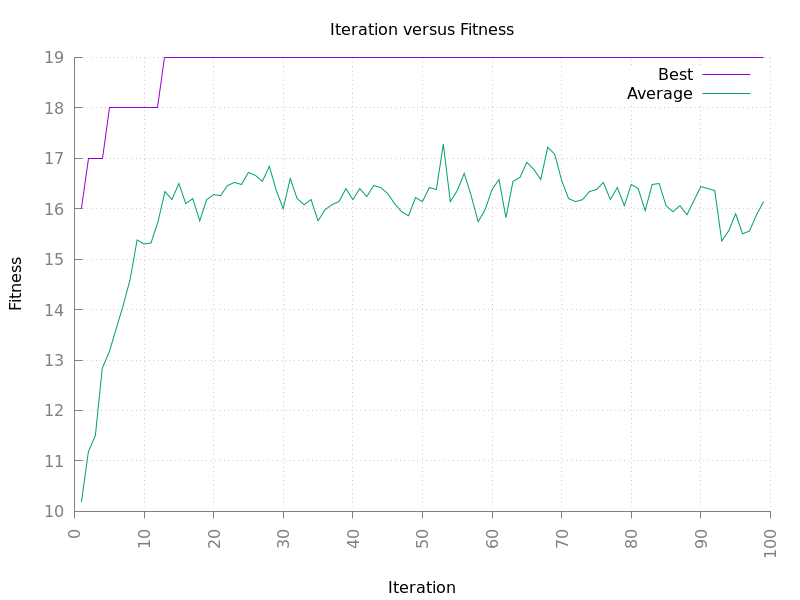
\includegraphics[width=.5\textwidth]{pictures/bin-alternate}
\end{figure}

O melhor indivíduo alcançou o fitness 19, o que era o ótimo nesse caso.

\subsection{Minimização da Função Esférica}

O objetivo é minimizar a função: $\sum^{n}_{i=1} i ^ 2$, sendo $n$ o tamanho escolhido para o gene de um indivíduo.

A função de adaptabilidade primeiramente calcula o valor do somatório, e retorna o  valor calculado, normalizado, 
armazenando o maior valor já encontrado pela população o subtraindo a função objetivo desse maior valor encontrado. 
Dessa maneira, quanto menor for o resultado do somatório, maior será o fitness.

\begin{figure}[h!]
    \centering
    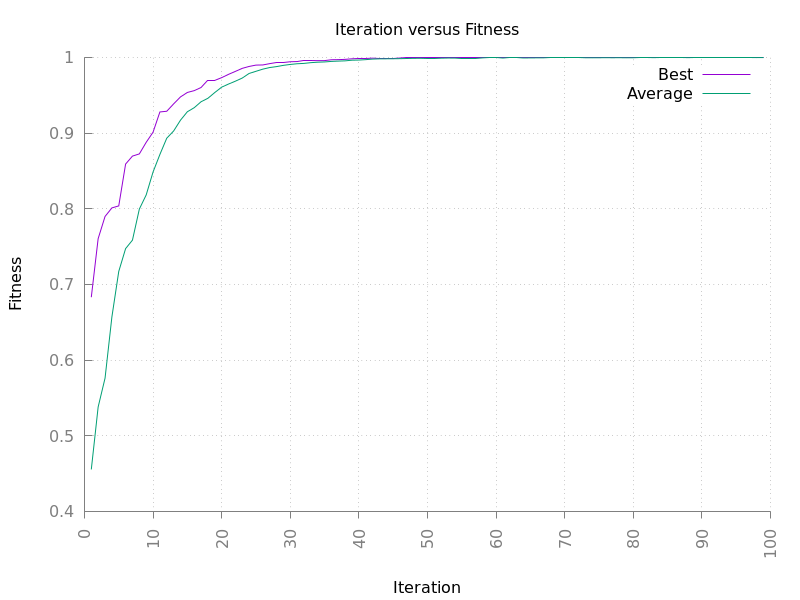
\includegraphics[width=.5\textwidth]{pictures/quadratic}
\end{figure}

Tanto o melhor indivíduo quanto a média foram capazes de convergir muito bem, foi utilizado a mutação delta com 
o crossover blx.

\subsection{Paridade Alternada}

Este problema é semelhante ao problema de bits alternados, a diferença é que neste a codificação da população 
é do tipo inteiro e é verificado se os elementos tomados a pares sequencialmente possuem paridades alternadas 
(par e ímpar ou ímpar e par).

A função de adaptabilidade itera sobre todo o gene do indivíduo e cada vez que encontra dois elementos com 
paridades alternadas acrescenta-se o \textit{fitness} em 1. Assim como o problema de bits alternados, 
se alcança o ótimo neste problema quando o \textit{fitness} do indivíduo for igual a $n - 1$, sendo $n$
o tamanho do indivíduo.

\begin{figure}[h!]
    \centering
    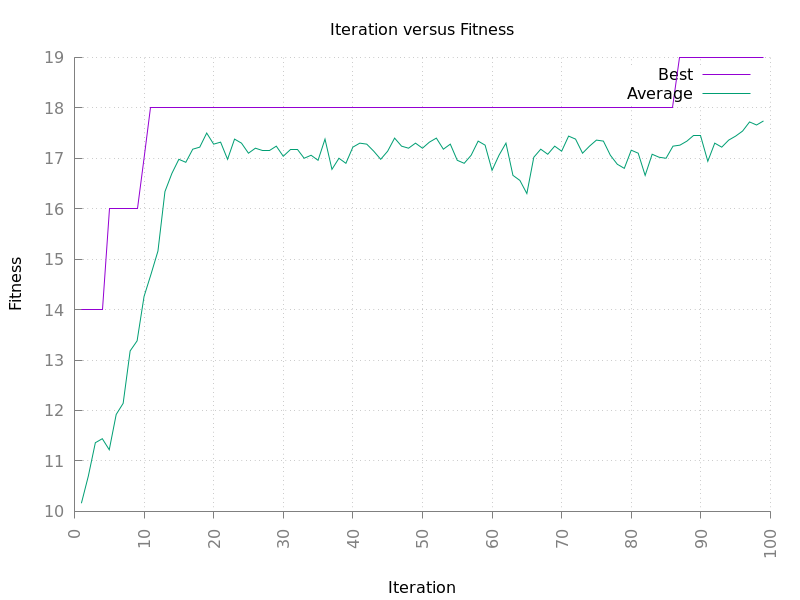
\includegraphics[width=.5\textwidth]{pictures/parity}
\end{figure}

Este foi o problema que mais demorou para convergir em 100 iterações para uma população de indivíduos de tamanho 20, 
foi utilizada a mutação delta adaptada para inteiros com o crossover uniforme, apesar da relativa demora para 
convergir, a média obteve um desempenho consistente.

\subsection{Maximização da Produção de Rádios}

Este problema é mais específico. O objetivo é maximizar o lucro com a produção de relógios, sendo que 
há dois tipos: normal e de luxo. Os normais fornecem um valor de 30 por unidade e os de luxo fornecem um 
valor de 40 por unidade. Os relógios normais necessitam de 1 homem-dia para serem produzidos e os 
relógios de luxo necessitam de 2 homens-dia para serem produzidos, sendo que a fábrica conta com 
40 homens-dia. 

Há um limite na quantidade de pessoas que podem trabalhar em cada uma das duas linhas, na de relógios 
normais é de 24 pessoas e na de relógios de luxo é de 32 pessoas, consequentemente, só podem ser 
produzidos 24 relógios normais e 16 relógios de luxo diariamente.

Para maximizar o lucro, a função objetivo é dada por $\phi = 30 * st + 40 * lx$, sendo $st$ o número 
de relógios normais e $lx$ o número de relógios de luxo. A função de adaptabilidade nesse caso é dada 
por: $f = \phi + r * h$, na qual $\phi$ é a função objetivo, $h$, é uma função de penalidade e $r$ é 
um coeficiente que representa o peso dado para a função de penalidade. Para este problema, o coeficiente 
escolhido foi -1.

Como este problema possui um limite de trabalhadores, há uma restrição dada por: $st + 2 * lx \leq 40$. 
Portanto, a função de adaptabilidade resulta em: \\ $f = 30 * st + 40 * lx - \max(0,st + 2 * lx - 40)$.

O max garante que o indivíduo não seja penalizado caso a quantidade de homens-dia não ultrapasse 40. 
Porém, ainda há um problema nessa modelagem, os valores não estão normalizados, desta maneira, é mais 
vantajoso violar a restrição do que obedecê-la, é necessário normalizar a função objetivo e a 
função de penalidade. O resultado final ficará: \\ \\ $f = \frac{30 * st + 40 * lx}{1360} - 
\max(0,\frac{st + 2 * lx - 40}{16})$.

Para resolver esse problema, foi utilizado uma população de indivíduos com codificação binária, com 
indivíduos de tamanho 10 (5 bits para representar a quantidade de relógios normais que varia entre 0 
e 24, e 5 bits para representar a quantidade de relógios de luxo, que varia entre 0 e 16).

No cálculo da função de fitness, o indivíduo primeiramente é dividido em dois vetores de tamanho 5, 
um para cada uma das duas variáveis do problema. Esses dois vetores de binários são convertidos para 
um valor em decimal, e este valor é normalizado para os limitantes de cada variável (0 a 24 e 0 a 16).

Com os valores das variáveis convertidos e normalizados, a função por fim calcula o \textit{fitness}
utilizando a fórmula supracitada, combinando as funções objetivo e de penalidade.

\begin{figure}[h!]
    \centering
    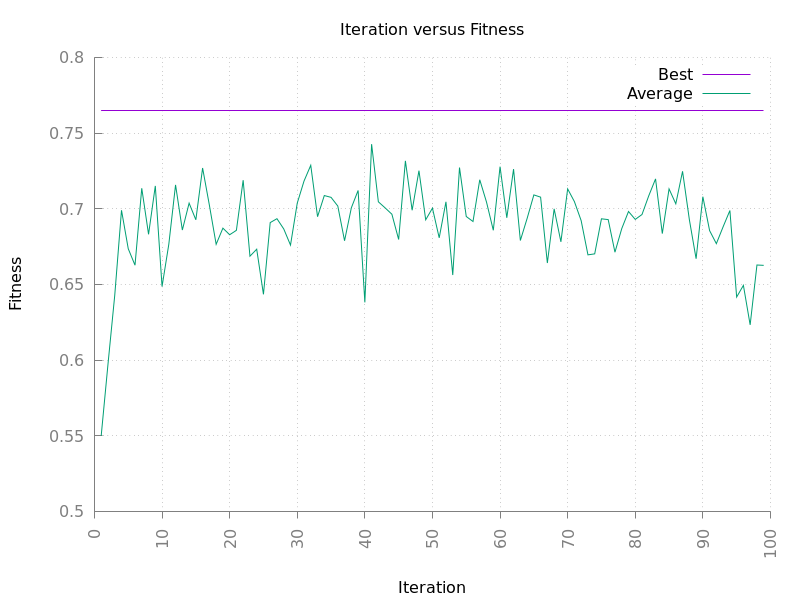
\includegraphics[width=.5\textwidth]{pictures/radio-factory}
\end{figure}

Coincidentemente já havia um indivíduo com a melhor solução na geração inicial, e como o elitismo 
foi utilizado, o melhor sempre permaneceu no topo. Considerando que nesse problema os indivíduos 
possuem tamanho 10, a convergência foi consideravelmente rápida, porém a média da população não 
se manteve consistente ao final da execução.

\subsection{Reconhecimento de Padrão Gráfico}

Para resolver esse problema, o padrão gráfico, por possuir apenas duas cores, foi transformado em um 
vetor de bits e a função de adaptabilidade simplesmente calcula uma distância de Hamming entre o 
padrão gráfico e o indivíduo e subtrai o resultado do número 36, que é o máximo que se pode 
atingir com essa operação.

Foi utilizado a mutação bit flip e o crossover uniforme.

\begin{figure}[h!]
    \centering
    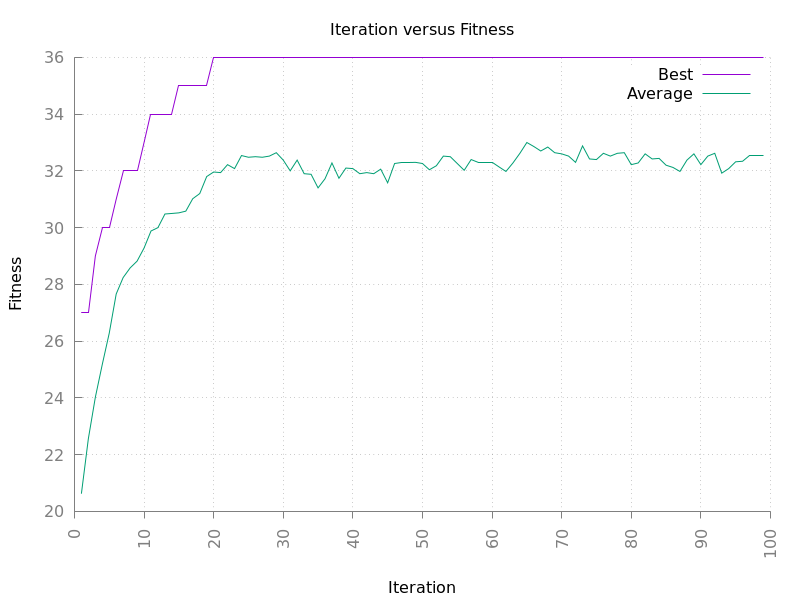
\includegraphics[width=.5\textwidth]{pictures/pattern-rec}
\end{figure}

Pode-se analisar que o melhor indivíduo foi capaz de atingir o ótimo, cujo valor da função objetivo 
deveria ser 36.

\bibliographystyle{sbc}
\bibliography{sbc-template}

\end{document}
